\documentclass[a4paper,12pt]{article}
\usepackage{graphicx}
\usepackage[T2A]{fontenc}
\usepackage[utf8]{inputenc}
\usepackage{csquotes}
\usepackage[russian,english]{babel}
\usepackage{apacite}
\usepackage{amsmath}
\usepackage{gensymb}
\usepackage[colorlinks,allcolors=cyan!70!black]{hyperref}
\title{Analysis of myosin-9-containing protein complexes in senescent MSCWJ-1 cells}
\begin{document}
\date{today}
\maketitle
\author[1,*]{Danila Bobkov}
\author[2]{Anastasia Polyanskaya}
\author[3]{Anastasia Musorina}
\author[4]{Ekaterina Lomert}
\author[5]{Sergey Shabelnikov}
\author[6]{Galina Polyanskaya}
%\author{Danila Bobkov, Anastasia Polyanskaya, Anastasia Musorina, Ekaterina Lomert, Sergey Shabelnikov, Galina Polyanskaya}
\affil[1,2,3]{Institute of Cytology of the Russian Academy of Science, 194064 Tikhoretsky ave. 4, St-Petersburg, Russia}

\section{Abstract}

Key words: mesenchymal stem cells, senescense, myosin-9

\section{Introduction}

At present, the urgent task of cell biology is the isolation and comparative characterization of human mesenchymal stem cells (MSCs) isolated from various sources. The importance of such studies stems from the features of the interaction of MSCs isolated from different tissues, with the characteristic microenvironment characteristic of each tissue. The origin or source of the MSC can determine their functional characteristics. Comparative analysis of the characteristics that are decisive in maintaining the status of MSCs, as well as a number of other characteristics responsible for the most important cellular processes, contributes to the deepening of basic knowledge of human MSCs, which is important both for understanding the mechanisms of biological processes in the cell and for expanding opportunities for using MSCs. in regenerative medicine.
Due to the importance of MSC for the functioning of the body, the mechanisms of MSC interaction with damaged tissues and organs are widely studied. It has been shown that one of the most important mechanisms of action of various MSCs on damaged tissues is their ability to migrate to these sites and exert a trophic action due to the secretion of bioactive factors that alter the microenvironment of damaged cells and, thereby, improving tissue repair. At present, the mechanisms of tissue repair using MSCs related to the production of cytokines and paracrine factors are widely discussed in the literature (Phinney, Prockop, 2007; Carvalho et al., 2011; Guiducci et al., 2011; Gruenloh et al., 2011; Huang et al., 2013; Luo et al., 2013; Ando et al., 2014; Hendijani et al., 2015 a, 2015b; Danieli et al., 2016; Julianto, Rindastuti, 2016; Teixeira et al., 2016; Vulcano et al., 2016; Zachar et al., 2016).
Non-immortalized cell lines undergo a process of replicative aging. Replicative aging is a complex process that can begin at the early passages and gradually increase in the process of long-term cultivation. It is characterized by a significant decrease or cessation of proliferation, shortening of telomeres, morphological changes, increased β-galactosidase activity, increased expression of the tumor suppressor genes, decreased DNA repair and antioxidant activity of aging cells, due to reduced expression of the corresponding genes, decreased differentiation potential, a number of epigenetic changes et al., 2008; Kuilman et al., 2010; Redaelli et al., 2012; Estrada et al., 2013; Savickiene et al., 2016; Danisovic et al., 2017; Koltsova et al., 2017, 2018; Alessio et al., 2018; Kry Lova et al., 2018; Niedernhofer et al., 2018; Truong et al., 2018; Yu et al., 2018;). It is important to emphasize that aging of MSCs may be associated not only with replicative aging, which can be traced during prolonged passaging of MSCs in vitro, but also with factors external to MSCs. Aging mechanisms affect both MSCs and microenvironment. In this regard, it is the interaction of MSCs and the microenvironment that ensures the age characteristics of MSCs (Sethe et al., 2006). One of the essential signs of replicative aging is a decrease in cell motility or cell migration (Geissler et al., 2012; Bertolo et al., 2015; Turinetto et al., 2016; Zhang et al., 2018). Violation of migration processes contributes to the deterioration of tissue repair. Therefore, to use MSCs in regenerative medicine, it is necessary to know the nature of the process of replicative aging in a particular line. Aging cultures are not suitable for biomedical work.
Cell migration occurs through close contact with the extracellular matrix, on which cells are spread, and depends on the organization of the actin cytoskeleton. In this regard, it is essential to study the role of aging in the organization of the cytoskeleton. There are a number of works describing molecular mechanisms and functional changes during the reorganization of the cytoskeleton during replicative aging in different human and animal cell types (Larsen et al, 2003, Le Clainche, Carlier., 2008; Wang, Jang., 2009; Geissler et al. , 2012; Özcan et al., 2016; Turinetto et al., 2016; Moujaber et al., 2019). Currently, studies on the effect of replicative aging on cytoskeleton reorganization are at the stage of accumulation of experimental results. It is of considerable interest to analyze the effect of replicative aging on cell motility and the reorganization of the actin cytoskeleton in the human MSC line, which has not been used in detail in such studies.

Currently, much attention is paid to the selection of MSCs from extra-embryonic organs, which are formed in the first weeks of pregnancy, because obtaining MSCs from these organs is not associated with a number of restrictions in obtaining MSCs from other tissues: an invasive method of production and ethical problems (Bongso, Fong, 2013). Previously, we obtained a non-immortalized human cell line from the Varton's jelly umbilical cord, called MSCWJ-1. The analysis of the main characteristics confirming the status of MSCs for it, according to the requirements of the International Society for Cellular Therapy (Dominici, 2006; Sensebé et al., 2010; Krylova et al., 2017). Thus, the objectives of this study are: 1. Analysis of replicative aging in the process of long-term cultivation of the MSCWJ-1 cell line. 2. ??



\section{MATERIALS AND METHODS}

K le t to and. A line of human mesenchymal stem cells obtained from Varton's jelly of the umbilical cord of the person (MSCWJ-1) was used in the work. The cell line was obtained and characterized in the Collective Medical Center "Collection of cultures of cells of vertebrates" of the IC of the Russian Academy of Sciences (St. Petersburg). MSCWJ-1 cells were cultured in growth medium containing 90\% DMEM / F12 medium (Biolot, Russia) and 10\% fetal bovine serum (FBS) (Hyclone, United States). Cells were cultured under conditions of 5\% CO2 at 37 $\degree$ C and humidity of 90\%. Microbiological analysis confirmed the absence of bacterial, fungal and mycoplasmal contamination in the resulting line.
 Morphology cells were performed using an inverted microscope (NICON, Japan).
The efficacy of the β-galactosidase enzyme was evaluated by the β-galactosidase enzyme activity. MSCWJ-1 cells were grown in 3.5 cm Petri dishes until subconfluent formation. Then the medium was removed and the cells were stained using a reagent kit (Senescence β-galactosidase staining kit; Cell Signaling, USA), according to the instructions. In cells entering the phase of replicative aging, the cytoplasm has a bright blue color. The analysis was performed using an inverted microscope (NICON, Japan) on the 6th, 1? M, 20th and 28th passages; The percentage of stained cells in percent was determined by counting at least 1000 cells in different fields of view at one time point. The results were processed statistically using Student's t-test. Differences were considered significant when the probability of the null hypothesis P <0.05.

Cell cultures: MSC WJ

Fibroblasts isolated from the Varton's jelly of the umbilical cord of a person.
The cultivation method is monolayer, the reseeding procedure consists in removing the cells with 0.25\% trypsin, the multiplicity of sieving is 1: 3 and its optimum density is 4.0-5.0x $10 ^ 6$ cells / ml in amtule.
Replicative cell aging

Evaluated by $\beta$-galactosidase enzyme activity. MSCWJ-1 cells were grown in 3.5 cm Petri dishes until subconfluent formation.
Then the medium was removed and the cells were stained using a reagent kit (Senescence $\beta$-galactosidase staining kit; Cell Signaling, USA) according to the instructions. In cells entering the phase of replicative aging, the cytoplasm has a bright blue color. The analysis was performed using an inverted microscope (NICON, Japan) at 9th, 20th and 28th passages. The proportion of stained cells (\%) was determined by counting at least 1000 cells in different fields of view at one time point. The results were processed statistically using Student's t-test. Differences were considered significant when the probability of the null hypothesis P <0.05.
Passage Number of cells Percentage stained for $\beta$-gal,\%
9 1025 6.00 $\pm$ 0.74
20 1149 26.30 $\pm$1.30
28 1260 44.00 $\pm$ 1.40

Immunofluorescence:
Glasses with flattened cells were fixed in a 3\% solution of paraformaldehyde for 10 minutes at room temperature and permeabilized in a solution of 0.1\% TritonX-100 for 10 minutes at room temperature, then the glass with cells was poured with 1\% BSA solution for 20 minutes . Rabbit polyclonal antibodies produced against the N-terminal peptide of the heavy chain of nonmuscle myosin IIA and mouse monoclonal antibodies produced against the high molecular weight isoforms of tropomyosin were used as the first antibodies. Goat antibodies to the Alexa fluor 488 rabbit antigens (Invitrogen, USA) were used as second antibodies. To visualize the actin cytoskeleton, cells were stained with rhodamine phalloidin for 20 min at room temperature. Preparations were made on Wednesday ProLong Gold antifade reagent containing DAPI. and analyzed on a confocal microscope Olimpus (Germany).

Colocalization analysis
The microscope initially captures images in a resolution of 72 dpi with a side of 1024, we took each image in the red and green channels, to determine the ROI manually traced the cells, from 9 to 14 in each group of measurements ..
The coefficients of Pearson, Spearman, Manders and Kendall colocalization were calculated using ImageJ version 1.52i using the Coloc 2 plugin (Schindelin et al., 2012).
However, Pearsons correlation coeff. It can be pretty noisy, it can be noisy, it can be lost, it can be lost. RBNCC for Replicate Based Noise Corrected Correlation and a patent has been applied for. Corrected Correlation for Accurate Measurements of Colocalization. Journal of Microscopy 230, 121-133 (2008) Adler, J., Pagakis, S.  Parmryd, I. Journal of Microscopy pairs corrupted by severe noise.
Journal of Mathematical Imaging and Vision 37, 204-219 (2010) Bergholm, F., Adler, J.  Parmryd, I.Journal of Mathematical Imaging and Vision


For further analysis,
the values of
the $\tau$-Kendall rank correlation coefficient
 were used.


The values of the correlation coefficient rxy were interpreted in accordance with the Cheddock scale:
Values of the correlation coefficient rxy Characteristic of correlation constraint
less than 0.1 no link
0.1-0.3 weak
0.3-0.5 moderate
0.5-0.7 noticeable
0.7-0.9 high
0.9-0.99 very high
\cite{tinevez2017trackmate}

\cite{mclean2018trajr}
Lyzing:
We obtained cell extracts from a monolayer cell culture grown on 14 Petri dishes 9 cm in diameter.
In order to prevent the destruction of multimolecular protein complexes, in the first stage the medium in the plates was replaced with medium containing 10 $\mu$M formaldehyde, incubated for 10 minutes at 37 $\degree$ C, then a solution of glycine at a concentration of 1.875 g per 200 ml was added to each cup PBS, incubated for 5-7 min at 37 $\degree$  C. Subsequently, we washed the cups after glycine with a solution of PBS and poured 20 $\mu$l of protease inhibitor and 1 ml of lysis buffer was left for 1 minute on ice.
Next, the method of sequential selection of cell extract was collected in the ependorf 1 ml of the sample. The final stage of lizing was centrifugation for 10 minutes at a speed of 12 thousand. Turns (how many G?) Per second and freezing of the samples at -80 $\degree$  C.

High performance liquid chromatography
For gel-chromatographic separation of cell lysates, an FPLC system (Pharmacia) was used.
Signal detection was performed using .. Millichrome A-02
Elution was performed with elution buffer (150 mM NaCl, 50 mM Tris, pH 7.5, 0.02\% NaN3).
The column was calibrated with the following set of proteins:
Protein Molecular (weight per vial) weight (Mr) Source Ovalbumin (50 mg) 43,000 Hen egg Conalbumin (50 mg) 75,000 Chicken egg white Aldolase1 (50 mg) 158,000 Rabbit muscle Ferritin1 (15 mg) 440,000 Horse spleen Thyroglobulin (50 mg) 669,000 Bovine thyroid Blue dextran 2000 (50 mg) 2,000,000 Aprotinin (10 mg) 6500 Bovine lung Ribonuclease A (50 mg) 13,700 Bovine pancreas Carbonic anhydrase (15 mg) 29,000 Bovine erythrocytes Ovalbumin (50 mg ) 43,000 Hen egg Conalbumin (50 mg) 75,000 Chicken egg white Blue dextran 2000 (50 mg) 2,000,000

Collected fractions on ice 1 ml.
100 $\mu$l of 0.15\% DOX sodium deoxycholate was added to the collected fractions and mixed vigorously, incubated for 10 minutes in a refrigerator, then 100 $\mu$l of 50\% TCA was added, mixed, incubated for 15 minutes in a freezer, and precipitated by centrifuging the protein for 30 minutes at 16000 RPM (G) at + 4 C.
The supernatant was removed, and cold 100\% acetone was added to the precipitate, mixed vigorously and incubated for 12 hours at -20 $\degree$C. A repeated washing with acetone was done, and then ..
The protein was then precipitated by centrifugation for 15 min at 16,000 RPM at + 4 $\degree$ C, the supernatant was collected, the precipitate was dried, and 2-fold sample buffer was added to the precipitate (125 mM Tris-HCl, pH 6.8, 4\% SDS, 10\% glycerol, 0.006\% bromo-phenol blue, 1.8\% $\beta$-mercaptoethanol).
Samples were boiled for 10 minutes at 98 $\degree$C.
Electrophoresis and western blot
Proteins were separated by electrophoresis in a 12.5\%  polyacrylamide gel under denaturing conditions in the presence of SDS (Laemmli, 1970).
After electrophoresis, the gel was stained with Coomassie brilliant blue or carried out by Western blotting (Towbin et al., 1979).
Protein transfer from the gel to the Immobilon-P membrane (Millipore, United States) was carried out in Tris-glycine buffer pH 8.3, containing 10\% ethanol and 0.1\% SDS.
Western blotting was performed according to the ECL protocol (Amersham, USA).
After transferring, the membrane was washed for 20 minutes with PBS containing 0.1\% tween-20 and blocked non-specific binding sites with 5\% non-fat dry milk diluted in PBS for 1 hour.
The membrane was incubated with the first antibodies for 1 hour at room temperature three times. washed in PBS, stained with second antibodies for 1 h at room temperature. Rabbit polyclonal antibodies produced against the N-terminal peptide of myosin-9, mouse monoclonal antibodies produced against the high molecular weight isoforms of tropomyosin, beta-actin, alpha-tubulin, or acetylated alpha-tubulin were used as the first antibodies.
Rabbit antibodies to mouse antigens and goat antibodies to rabbit antigens conjugated with horseradish peroxidase (Sigma, USA) were used as second antibodies.
To enhance the signal in western blotting, SuperSignal substrate (Thermo Scientific, USA) was used.
Chemiluminescent radiation was recorded using a ChemiDoc system (Bio-Rad, USA).
Densitometry of blots was performed using the ImageJ program (Schindelin et al., 2015), and statistical analysis of the densitometry data was performed using Microsoft Excel.

Description of statistical analysis methods
The study materials were subjected to statistical processing using the methods of parametric and non-parametric analysis. The accumulation, correction, systematization of the initial information and visualization of the obtained results were carried out in Microsoft Office Excel 2016 spreadsheets.
Statistical analysis was carried out using the free software computing environment R v. 3.5.3 (\cite{team2014r}).
The data obtained from measurements of the colocalization coefficient were combined into variational series, in which the arithmetic mean values (M) and standard deviations (SD) were calculated, the limits of the 95\% confidence interval (95\% CI).
Quantitative indicators were evaluated for compliance with the normal distribution, for this purpose, the Shapiro – Wilk criterion [6, 7] was used (with 8 <n <15).
as well as indicators of asymmetry and kurtosis.
When comparing several samples of quantitative data with a distribution other than normal, Kruskal-Wallis criterion was used, which is a non-parametric alternative to single-factor analysis of variance. The Kruskal-Wallis criterion was calculated after ranking all the elements of the analyzed sets by the following formula:



where H is the Kruskal-Wallis criterion, n is the total number of measurements, Ri is the sum of the ranks of measurements related to a particular sample, k is the number of matched samples.
In the event that the calculated value of the Kruskal-Wallis criterion exceeded the critical one, the differences in the indicators were considered statistically significant. Otherwise, the null hypothesis was recognized true.
When comparing the mean values in normally distributed sets of quantitative data, the Student’s t-test was calculated using the following formula:

where: M1 and M2 are compared average values, m1 and m2 are standard errors of average values, respectively. The resulting values of Student's t-test were evaluated by comparing with critical values. Differences in indicators were considered statistically significant at a significance level of p <0.05.

Multiple Testing Correction
In the course of multiple pairwise comparisons, the Bonferroni method, the Benjamin-Yekuteli-Hochberg method (FDR) was used to adjust the P-values.
the results were visualized using the free Python computing software environment and the scikit-posthocs package (Terpilowski, 2019).
We also used the Wilcoxon W-test to check the differences between the two paired samples compared. At the same time, for each group of measurements, the magnitude of the change in the colocalization coefficient was calculated. All changes were ordered in absolute value (excluding the sign). Then ranks were assigned a change sign (“+” or “-”), for each sign the ranks were summed. A smaller sum of ranks (W) was selected, which was compared with the critical value of the W-criterion. If the calculated value of W was less than or equal to the critical value, it was concluded that the differences of the compared samples were statistically significant.



\section{RESULTS}

1. Immunofluorescent cell analysis
When stained with antibodies against myosin heavy chain ...
In fig. 2 shows cells ..
Myosin-9 is distributed along stress-fibrils, striation is often observed along stress-fibrils,

Morphological analysis of the cell line during long-term cultivation showed homogeneity of cell populations with medium-sized elongated fibroblast-like cells at the 9th and 28th passages (Fig. 1, a, b,). In the process of cultivation, there is a change in the morphology of the cells, expressed in an increase in the size and degree of cell spreading.
The process of replicative aging during long-term cultivation of cells of all lines was assessed by the activity of $\beta$-galactosidase in cell populations (Table 1).


Table 1

\begin{figure}[hbt!]
\centering
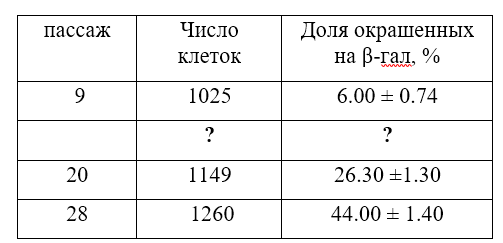
\includegraphics[width=0.6\linewidth]{tab.png}
\caption{The proportion of cells with pronounced activity of $\beta$-galactosidase ($\beta$-gal)
 in the process of cultivating the MSCWJ-1 line}
\label{fig:tab}
\end{figure}

Note. Given the mean values and their errors when counting at least 1000 cells in different fields of view at one time point. The difference between the early and late passages for both lines is significant (P <0.05).
  From the results of Table 1, it follows that in the MSCWJ-1 line, the process of replicative aging begins with?


\begin{figure}[hbt!]
\centering
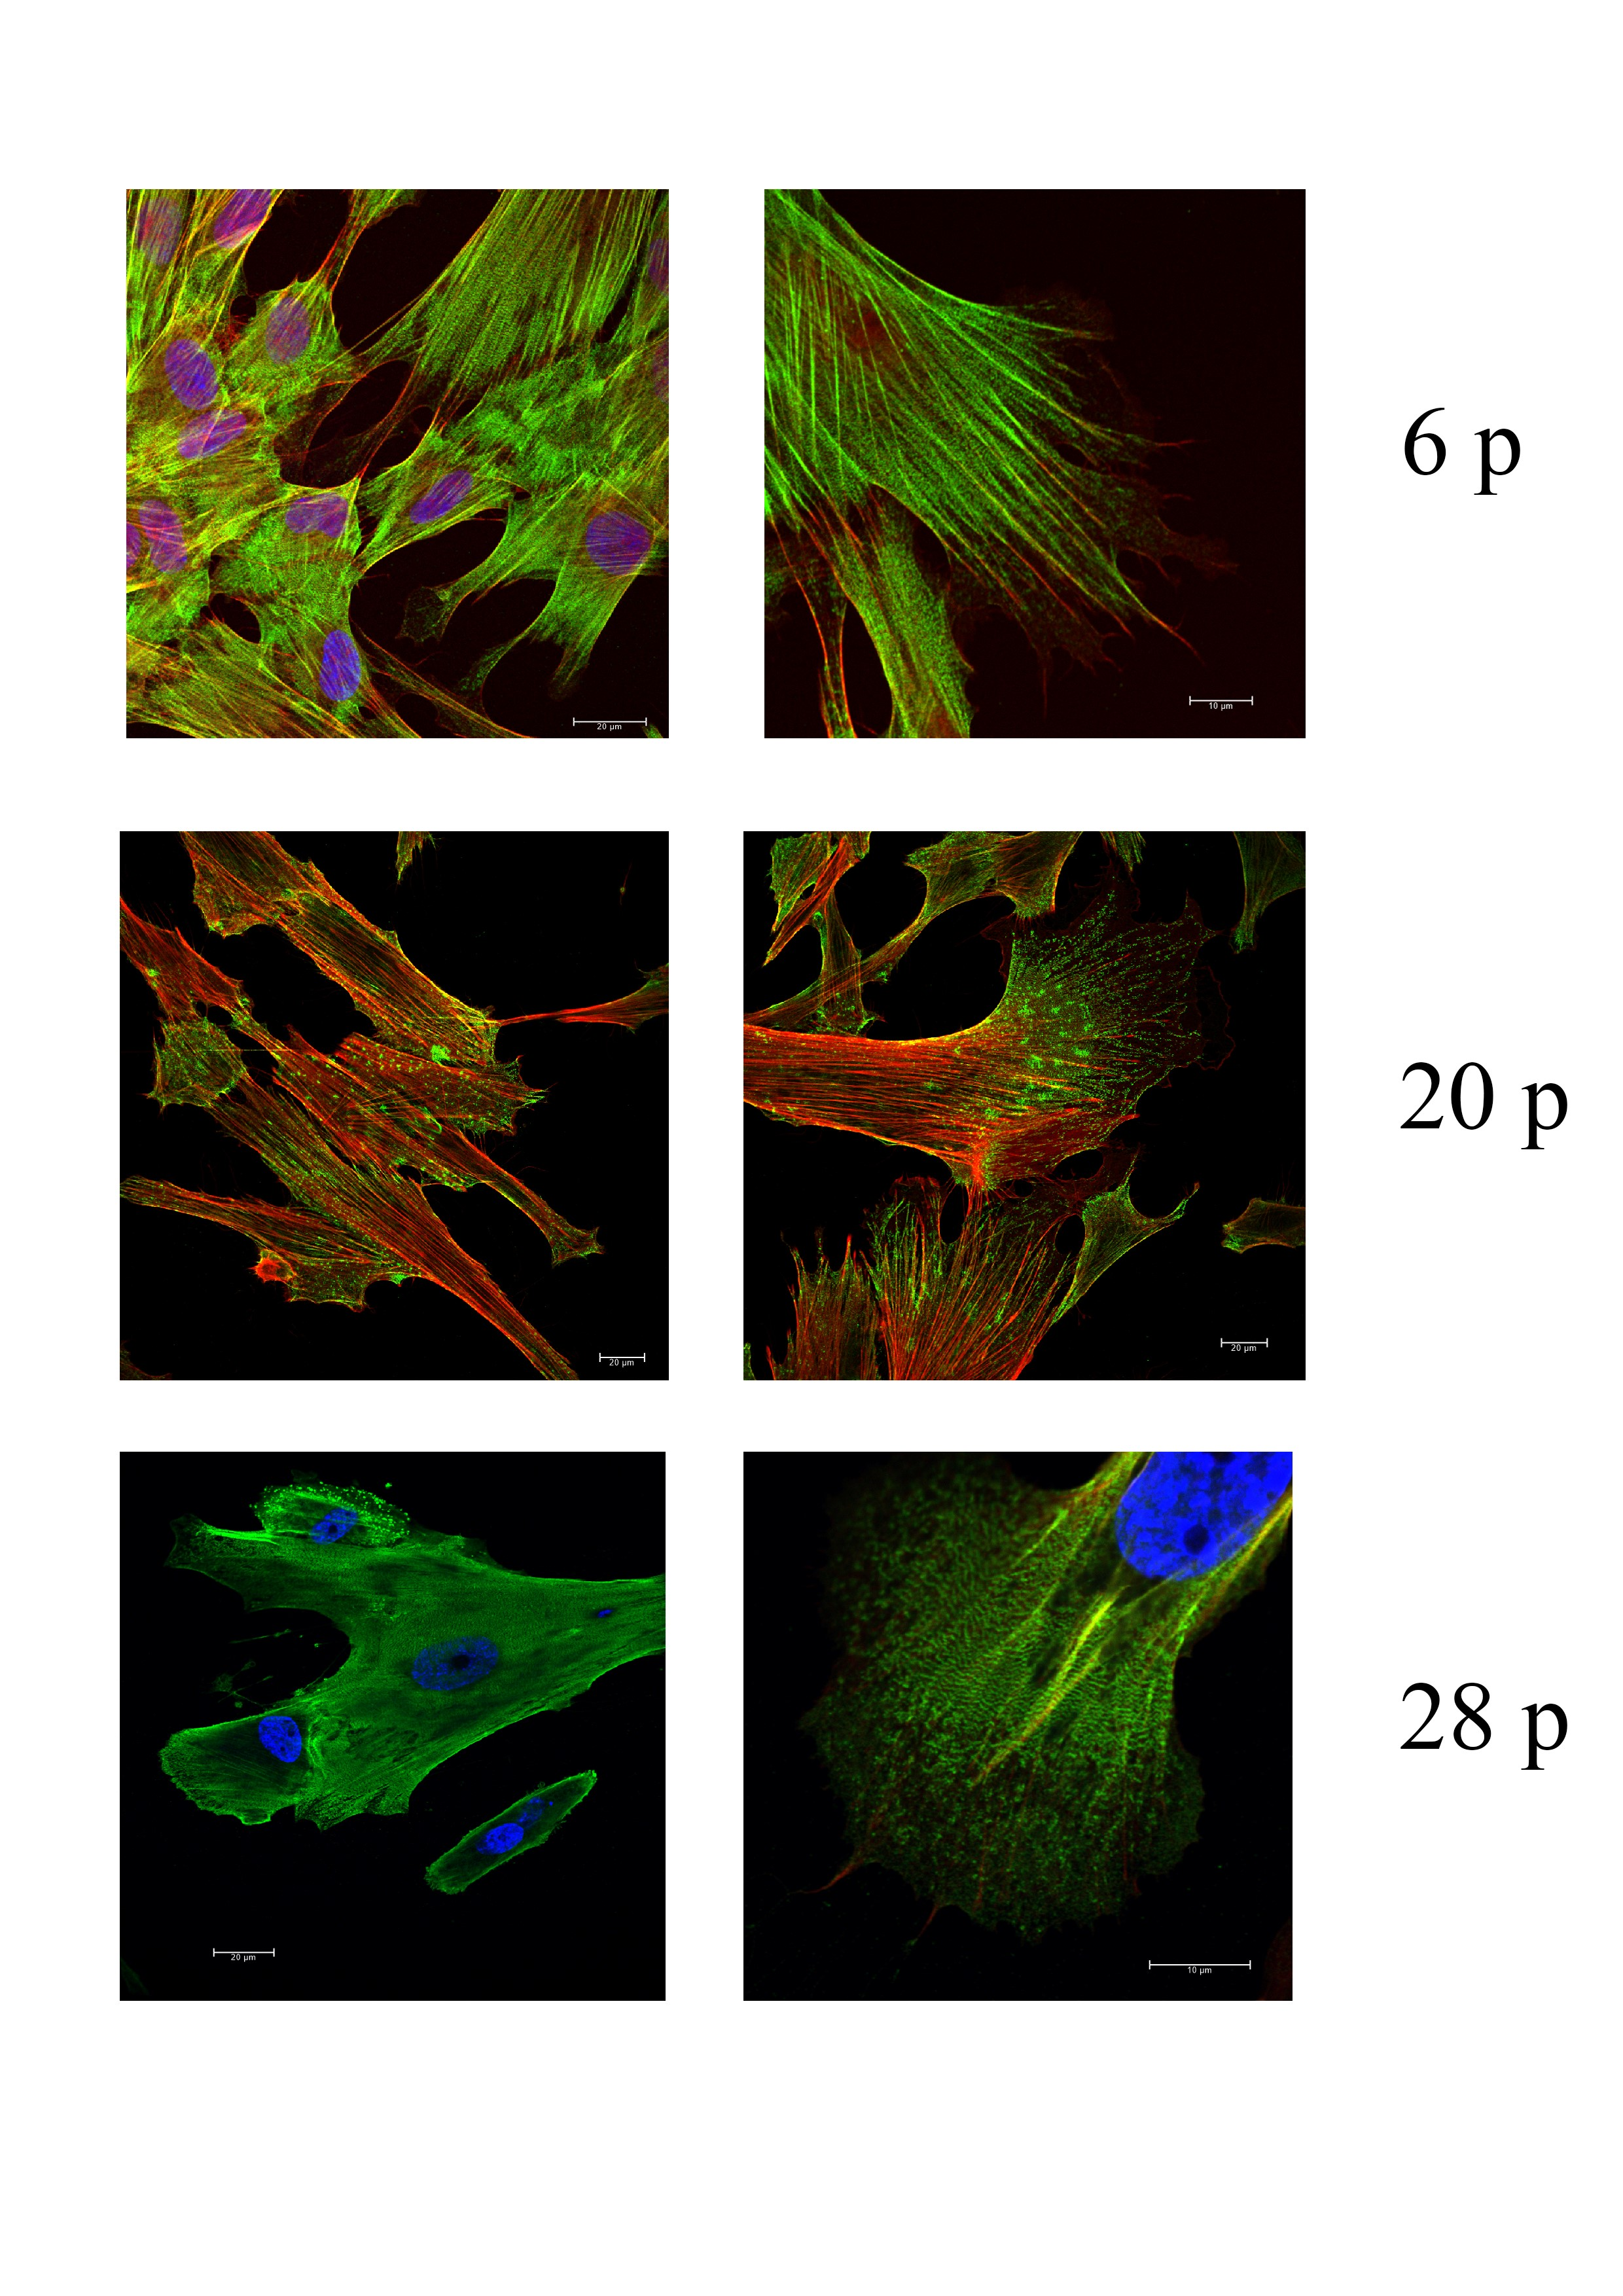
\includegraphics[width=0.6\linewidth]{fig1.jpg}
\caption{Different passages staining of F-actin (red) and myosin-9 (green)}
\label{fig:fig1}
\end{figure}

\begin{figure}[hbt!]
\centering
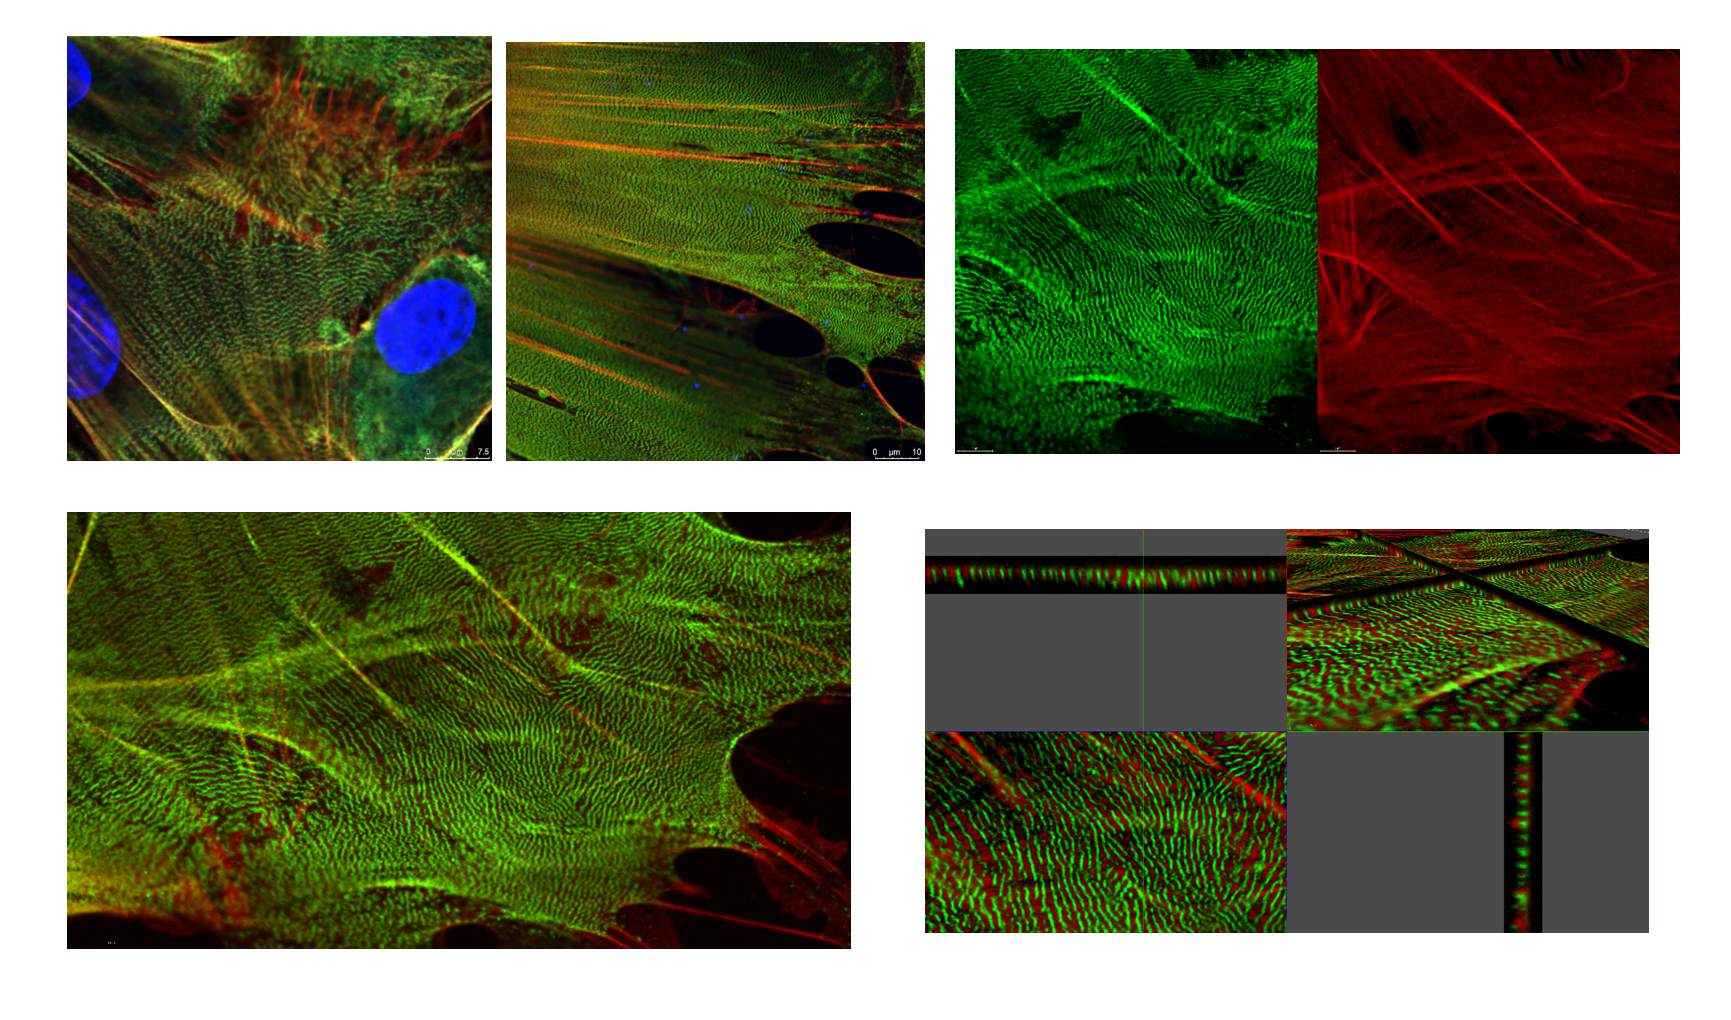
\includegraphics[width=0.6\linewidth]{fig7.png}
\caption{Different passages staining of F-actin (red) and myosin-9 (green)}
\label{fig:fig7}
\end{figure}

Fig.1. Confocal microscopy of fixed cells ..., at different passages ... 6 p - cells at 9 passage. Red - rhodamine-phalloidin, green - myosin-9, blue - core

\begin{figure}[hbt!]
\centering
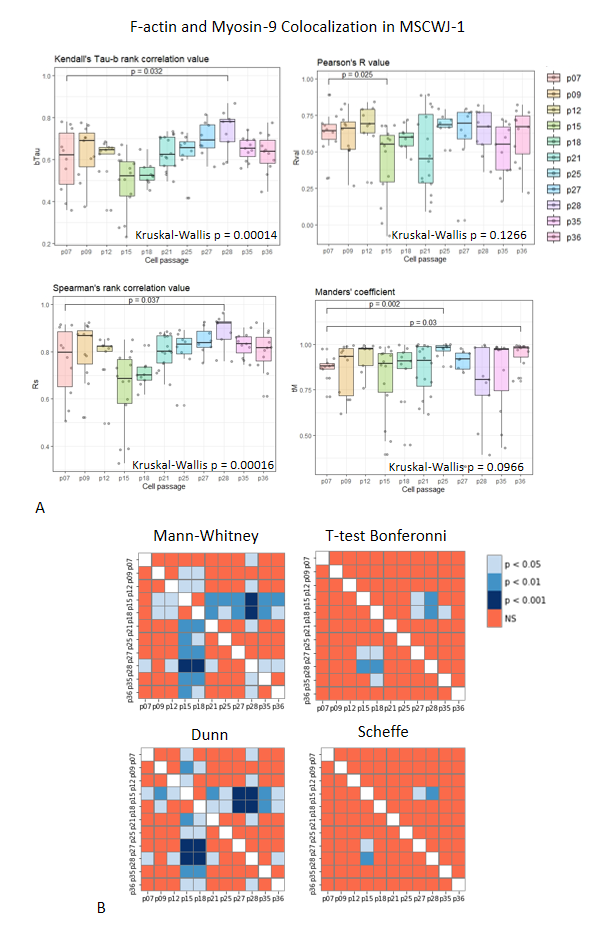
\includegraphics[width=0.6\linewidth]{fig2.png}
\caption{Different passages staining of F-actin (red) and myosin-9 (green)}
\label{fig:fig2}
\end{figure}

Fig.2. Kendal Miozin-9 and F-actin colocalization coefficient in р7-28р. Mean and standard error, Dynamics with confidence intervals, significant difference between groups. Pairwise t-test and t-test with Bonferroni correction

Colocalization of proteins

To check the data for normality, we applied the Shapiro-Wilk criterion.
The results of the Shapiro-Wilk test for measurements are presented in the table:
...
The results of the Shapiro-Wilk test indicate that the distribution of the values of the tau-Kendall rank correlation coefficient is not statistically significantly different from the normal (p> 0.05) in all groups of measurements. A multiple comparison of the medians of all samples was performed using the Kruskal-Wallis test, his results (chi-squared = 30.751, df = 8, p-value = 0.0001556) allowed to reject the null hypothesis and to conclude that there is a significant difference between the samples.
 During the post hoc analysis, we used parametric Student’s two-sample t-test for independent samples to check the differences between paired samples of independent measurements by the level of the tau-Kendall rank correlation coefficient.
However, in the Shapiro-Wilk test, the p-value for the p25 sample turned out to be 0.05657, which is only slightly higher than the significance criterion chosen by us. At the same time, quantile plots show deviations from normality for high and low index values (Fig.).
Therefore, to eliminate doubts about the normality of the data, we also used the non-parametric Wilcoxon sign rank test to check the differences between paired samples of independent measurements by the level of the tau-Kendall rank correlation coefficient.



\begin{figure}0.0929
  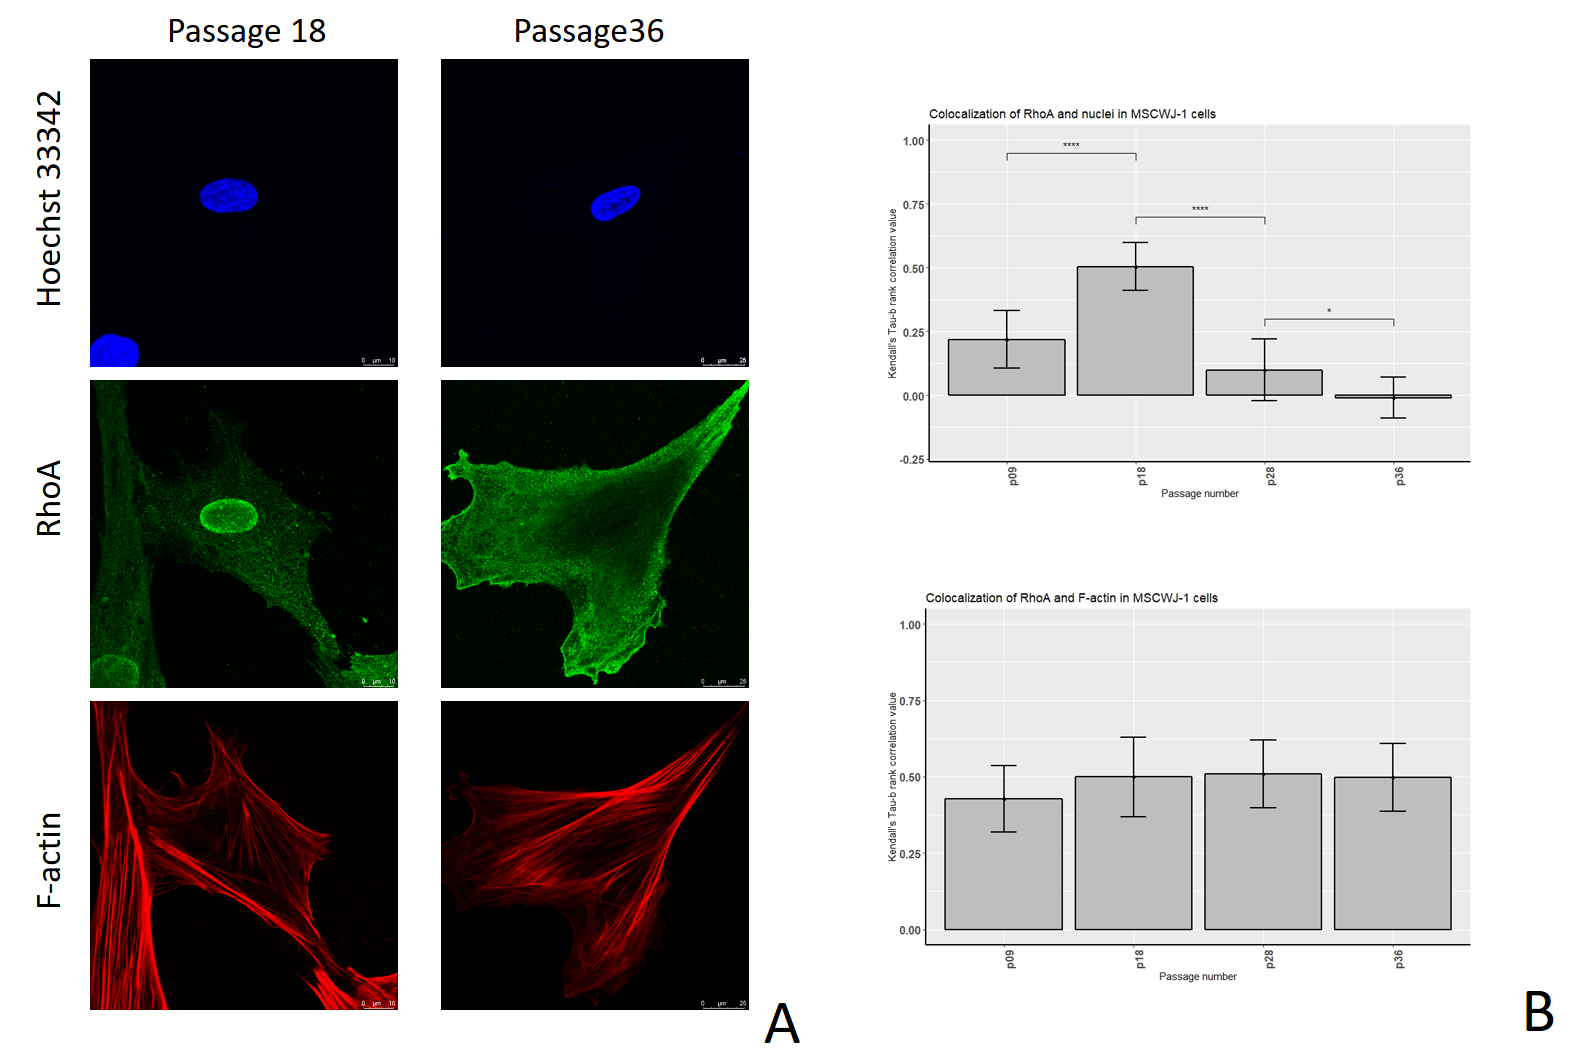
\includegraphics[width=0.6\linewidth]{fig3.png}
  \caption{Fig.3. RhoA in the nucleus, along the stress In the perinuclear region, diffusely in the cytoplasm}
  \label{fig:fig3}
  \centering
\end{figure}

Figure \ref{fig:fig3} shows aRhoA in the nucleus...

\begin{figure}[hbt!]
\centering
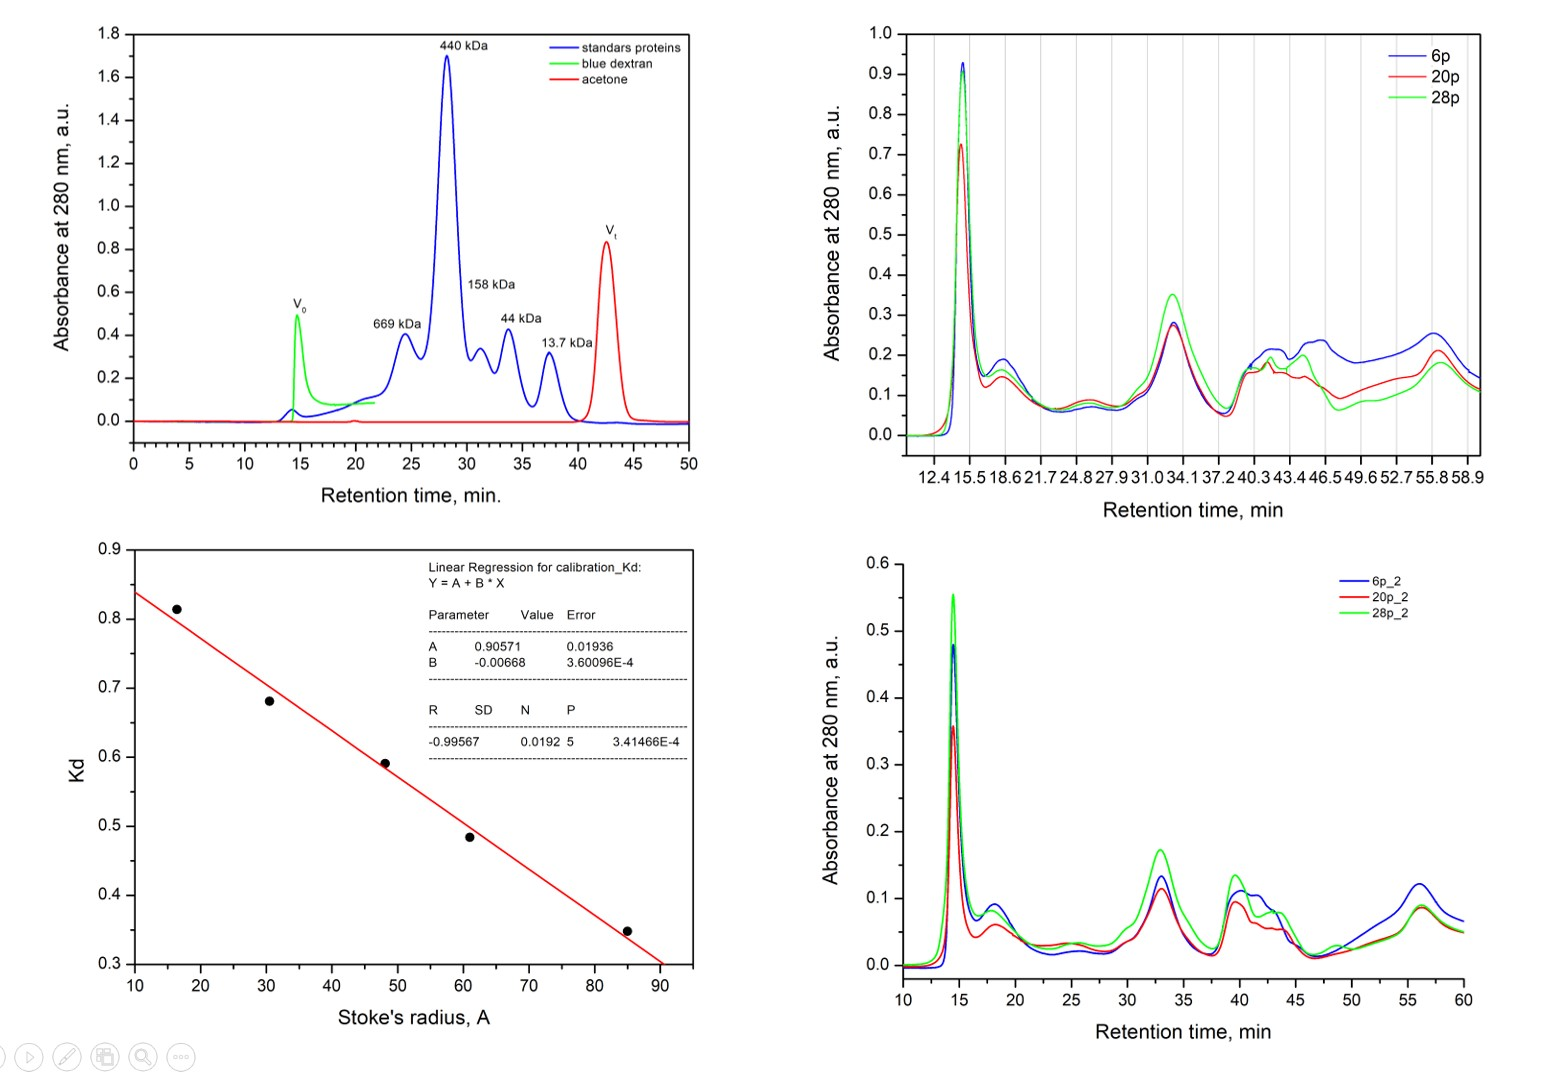
\includegraphics[width=0.6\linewidth]{fig4.jpg}
\caption{Fig. 4. Gel chromatographic separation of cytoplasmic extracts from WJ1 cells at different stages of replicative aging. Separation of calibration proteins (A) and comparison of elution profiles are presented.}
\label{fig:fig4}
\end{figure}

\begin{figure}[hbt!]
\centering
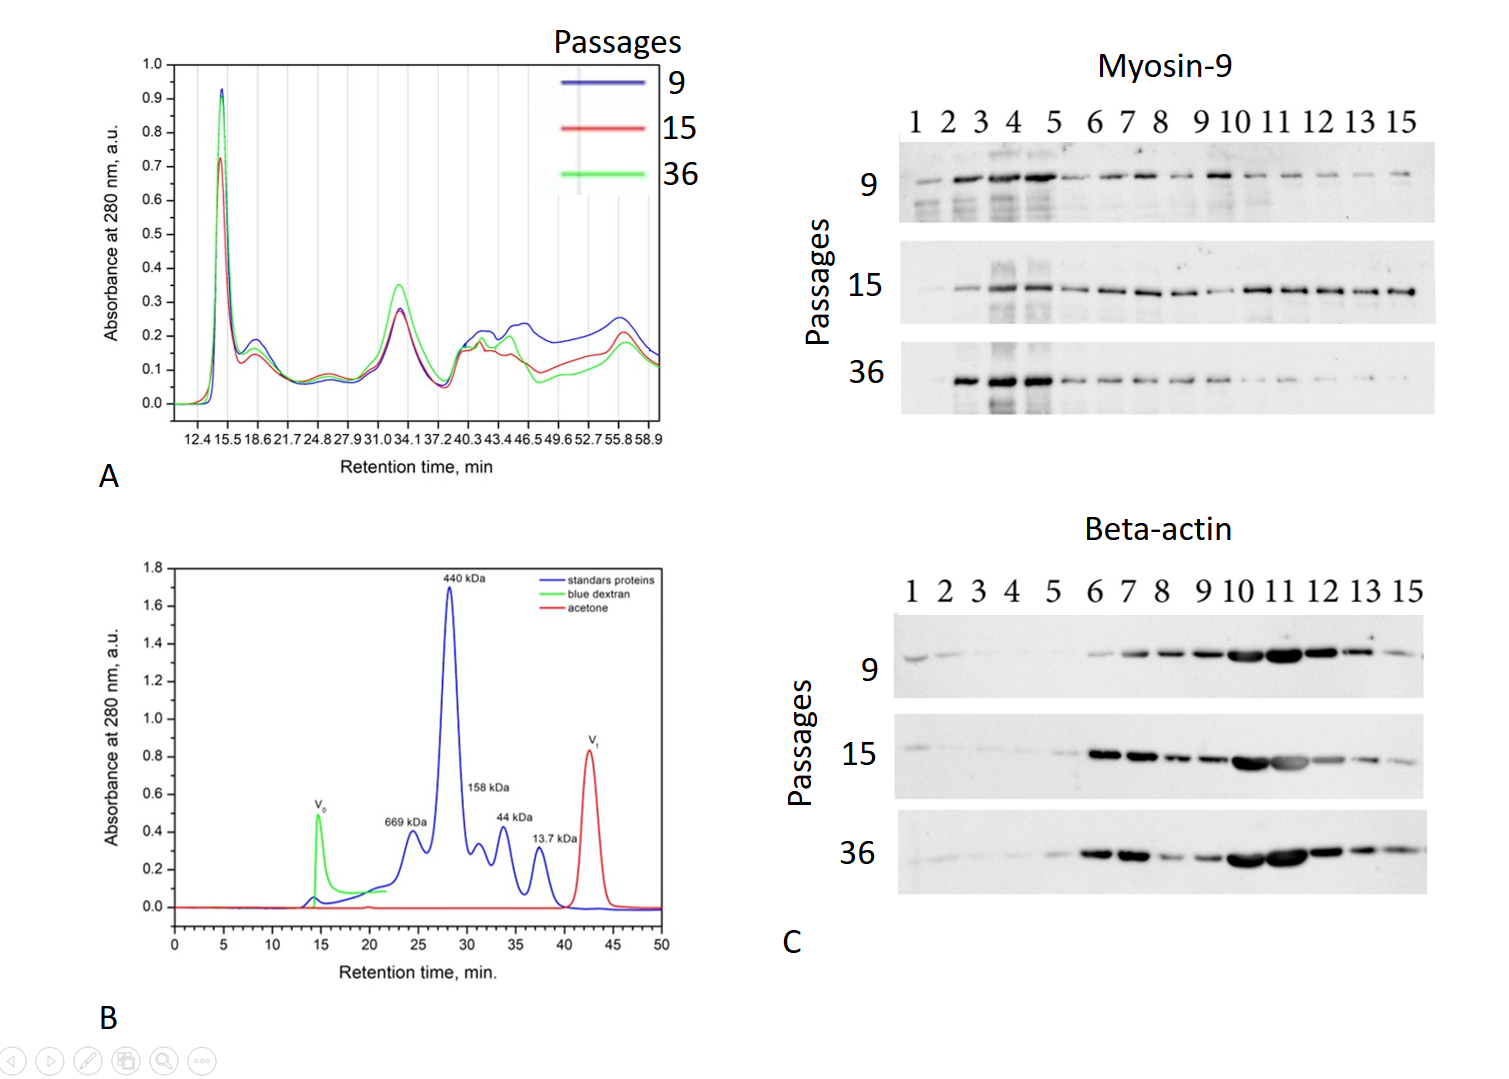
\includegraphics[width=0.6\linewidth]{fig5.png}
\caption{Fig.5 Electrophoretic separation of proteins from fractions obtained as a result of gel-chromatographic separation of cytoplasmic extracts from WJ1 cells in various stages of replicative aging.}
\label{fig:fig5}
\end{figure}

Pic.6 Western blot and densitometry



\section{DISCUSSION}

The actin cytoskeleton and its associated motor proteins provide the driving forces for creating amazing morphological diversity and the dynamics of mammalian cells.

Such as maintaining cell shape, its migration, interaction with the substrate and with other cells, cytogenesis, processes of intracellular transport, as well as participation in the conduct of the cellular signal and the regulation of gene expression.
Cellular actin cytoskeleton appears
the globular actin assembly mechanism (G-actin) into threads consisting of double helix (F-actin).
Assembling and disassembling F-actin is a very dynamic process to perform various functions of actin. Similar dynamics are regulated by a number of actin-binding and regulatory proteins.
Thus, there are mechanisms that prevent the spontaneous polymerization of G-actin into filaments by the relative instability of actin dimer or trimer and G-actin-binding and sequestering proteins, such as profilin and $\beta$-thymosin, respectively (....).
On the other hand, a number of actin-binding proteins prevent the depolymerization of F-actin microfilaments and regulate their stability (such as tropomyosin, alpha-actinin, for example). A recent study has shown that targeting and activation of actin filament nucleators (gelsolin), elongators, and myosin engines are closely coordinated by conservative protein complexes to orchestrate the generation of power. (Pantaloni and Carlier, 1993; Sept and McCammon, 2001; Xue and Robinson, 2013). The distribution of these and many other structures in the cell allows you to perform all the variety of the above functions.
the above listed functions.
To establish the many different actin assembly functions required in time and space, actin nucleators target specific subcellular compartments, thereby limiting the formation of specific structures of actin filaments to these sites.
Cellular aging, replicative cycle, Hayflick limit
Currently, two main theories about the mechanisms of aging are competing with each other: telomeric and oxidative (it is free radical, it is mitochondrial). In 1961, an American doctor, Leonard Hayflick, discovered that human cells cannot endlessly divide: in vitro they undergo approximately 50 doublings and stop proliferation (Hayflick, Moorhead, 1961). This figure of 50 doublings, called the Hayflick limit, is fairly arbitrary, since it is not possible to accurately determine how many times a single human cell can share. Thus, the results of Hayflick's experiments do not mean that the human cell is able to share exactly 50 times (most likely more), but only mean that with the counting method that Hayflik used and which is used now as the simplest and most convenient, a population of human fibroblasts in culture doubles usually ~ 50 $\pm$ 10 times.
Cell cycle arrest during replicative aging

Another structure characteristic mainly of non-muscle cells is stress fibrils — bundles of F-actin filaments stabilized by such proteins, ...
Features of the organization of the actin cytoskeleton in mesenchymal stem cells
The most important population of adult stem cells are mesenchymal stem cells (MSCs). For the first time, these cells were detected and isolated from the bone marrow stroma. It was believed that bone marrow MSCs serve as a source for the renewal and restoration of connective tissues such as bone, cartilage and adipose. At present, analogs of bone marrow MSC are found in all other tissues. Thanks to the approaches that allow identifying MSCs in situ, isolating them from tissues and finally evaluating biological properties, it became possible to revise the role of MSCs in various organs and tissues. This review summarizes our own and published data on the role of MSCs in the processes of repair and tissue regeneration. In our opinion, MSCs perform the function of conjugating the circulatory, immune, hormonal, and nervous systems with tissue-specific stem cells.


Elliott et al. find that Rho/ROCK-stimulated myosin II contractility minimizes cell-scale branching by recognizing and minimizing local cell-surface curvature \cite{elliott2015myosin}.

Differences in the organization of the cytoskeleton in normal and cancer cells. Shutova MS, Aleksandrova A. Yu. Comparative study of the spreading of normal and transformed fibroblasts. The role of microfilament polymerization and actin-myosin contraction // Tsitol. - 2010. - T. 52. - №. 1. - p. 41-51.
The cell movement is based on the rearrangement of the actin cytoskeleton. The initial step of the rearrangements is the formation of the so-called leading (active) edge, at which protrusions take place and primary contacts of the cell with the extracellular matrix are formed. Protrusion of the leading edge is provided by the force of polymerization of actin in the zone of the lamellipodia. In the lamella zone, a further rearrangement of actin takes place - the formation of actin-myosin beams. The formation of contacts with the substrate is initiated in the lamellipodia, and maturation occurs in the lamella zone with the participation of stress-fibrils (Bershadsky et al., 2006; Alexandrova et al., 2008). The tension generated by myosin affects the initial focal complexes, inducing their growth and transformation into focal contacts (Ingber, 1991; Riveline et al., 2001; Rottner et al., 2001; Krendel, Mooseker, 2005) .
A striking example of the dynamic organization of the cytocell is its restructuring, occurring in the cell spreading process. The process of spreading begins with the formation of pseudopodia around the entire perimeter of the cell. The network of microfilaments on the active edge is constantly formed during the entire spreading process due to the intense polymerization of actin. The remaining types of actin-containing structures arising in sprawling cells are mainly the result of a sequential reorganization of actin polymerized at the edges. The first stage of such a rearrangement is the emergence of an annular beam located along the edge of the discoid cell immediately behind the zone of the active edge (radial spreading stage) (Svitkina et al., 1986). In the case of fibroblast-like cells, the spreading process on the substrate ends with the stage of polarization. Fibroblasts acquire an elongated polarized form as a result of the redistribution of pseudopodial activity - the division of the cell edge into active and stable zones (Rivne, Vasiliev, 2004).
Neoplastic transformation disrupts normal morphogenetic reactions and cell mobility, leading to processes such as invasive growth and metastasis (Rovno, Vasiliev, 2004). Reorganization of the cytoskeleton, especially changes in cell contractility, regulated by the actin-myosin complex, is of central importance for the development of the phenotype of morphologically transformed cells with invasive behavior. The reduction of stress-fibrils, characteristic of many types of transformed cells, is associated with impaired maturation of contact structures (Rovno, Vasilyev, 2004) and often correlates with an increase in locomotor activity and / or metastatic potential of tumor cells (Pokorna et al ., 1994; Sahai, Marshall, 2002). The transformed cells in the culture are observed violations of spreading. At all stages of spreading, the distribution of lamellipodia is disturbed, as a result of which lamellae are formed as separate fragments, and not along the entire perimeter of the cell. Flattening of the cell is uneven, disc-shaped is not observed. Upon completion of the spreading, such cells do not reach a large area comparable to the area of normal cells (Rovensky, Vasiliev, 2004).

\cite{vicente2009non}




\section*{Conclusion}

Sed ut perspiciatis unde omnis iste natus error sit voluptatem accusantium doloremque laudantium, totam rem aperiam, eaque ipsa quae ab illo inventore veritatis et quasi architecto beatae vitae dicta sunt explicabo.

Replicative aging of human mesenchymal stem cells is accompanied by changes in the organization of the contractile apparatus.

\section*{Author Contributions}

Author2 designed the research. Author1 carried out all simulations, analyzed the data. Author1 and Author2 wrote the article.

\section*{Acknowledgments}

We thank G. Harrison, B. Harper, and J. Doe for their help.

\bibliographystyle{apacite}
\bibliography{mybib.bib}
\end{document}
